\documentclass[degree=doctor,secret]{cugthesis}
% 选项:
%   degree=[bachelor|master|doctor|postdoctor], % 必选
%   secret,                                     % 可选
%   pifootnote,                                 % 可选(建议打开)
%   openany|openright,                          % 可选,基本不用
%   arial,                                      % 可选,基本不用
%   arialtoc,                                   % 可选,基本不用
%   arialtitle                                  % 可选,基本不用

% 所有其它可能用到的包都统一放到这里了,可以根据自己的实际添加或者删除。
\usepackage{thuthesis}
\usepackage{threeparttable} %三线表,带表注释

%**************************一些使用量很高的变量定义**********************************
\def\ca{{\text{Ca}^{2+}}}   			%公式: 使用时必须放在$$内当公式用
\def\so4{{\text{SO}_4^{2-}}}
\def\anhydrite{$\text{CaSO}_4$}         %硬石膏的化学式
\def\pyrite{$\text{FeS}_2$}                   %黄铁矿的化学式
\def\chalcopyrite{$\text{CuFeS}_2$}    %黄铁矿的化学式
\def\cca{$C_{\ca}$} 					        %Ca的浓度
\def\cso4{$C_{\so4}$}                        %SO4的浓度
\def\cfe{$C_{\text{Fe}}$}                  %Fe的浓度
\def\cs{$C_{\text{S}}$} 					   %S的浓度
\def\ccu{$C_{\text{Cu}}$}                    %Cu的浓度
\def\ksp{$K_{sp}$}                                   %Ksp
\def\ssd{$^{\circ}$C } 			%摄氏度:直接使用,最好后面空一格
%****************************************************************************************

% 定义所有的图片文件在 figures 子目录下
\graphicspath{{figures/}{../../figures/}}

% 可以在这里修改配置文件中的定义。导言区可以使用中文。

\begin{document}


%%% 封面部分
\frontmatter
\thusetup{
	%******************************
	% 注意:
	%   1. 配置里面不要出现空行
	%   2. 不需要的配置信息可以删除
	%******************************
	%
	%=====
	% 秘级
	%=====
	secretlevel={秘密},
	secretyear={10},
	%
	%=========
	% 中文信息
	%=========
	ctitle={ xxxx热液xxxxxx研究},
	cdegree={理学博士},
	cuniversity={中国地质大学},
	euniversity={China University of Geosciences},
	cdepartment={地球物理与空间信息学院},
	cmajor={地球物理学},
	cauthor={郭志馗},
	studentnum={22015xxxxx},
	csupervisor={xx教授},
	cassosupervisor={xxx研究员}, % 副指导老师
	ccosupervisor={xx Rüpke 教授}, % 联合指导老师
	cproject={国家留学基金委},
	% 日期自动使用当前时间,若需指定按如下方式修改:
	% cdate={超新星纪元},
	%
	% 博士后专有部分
	cfirstdiscipline={计算机科学与技术},
	cseconddiscipline={系统结构},
	postdoctordate={2009年7月——2011年7月},
	id={编号}, % 可以留空: id={},
	udc={UDC}, % 可以留空
	catalognumber={分类号}, % 可以留空
	%
	%=========
	% 英文信息
	%=========
	etitle={Numerical simulation xxxxxx},
	% 这块比较复杂,需要分情况讨论:
	% 1. 学术型硕士
	%    edegree:必须为Master of Arts或Master of Science(注意大小写)
	%             “哲学、文学、历史学、法学、教育学、艺术学门类,公共管理学科
	%              填写Master of Arts,其它填写Master of Science”
	%    emajor:“获得一级学科授权的学科填写一级学科名称,其它填写二级学科名称”
	% 2. 专业型硕士
	%    edegree:“填写专业学位英文名称全称”
	%    emajor:“工程硕士填写工程领域,其它专业学位不填写此项”
	% 3. 学术型博士
	%    edegree:Doctor of Philosophy(注意大小写)
	%    emajor:“获得一级学科授权的学科填写一级学科名称,其它填写二级学科名称”
	% 4. 专业型博士
	%    edegree:“填写专业学位英文名称全称”
	%    emajor:不填写此项
	edegree={Science},
	emajor={Geophysics},
	eauthor={Zhikui Guo},
	esupervisor={Prof. Dr. xx},
	eassosupervisor={Prof. Dr. xx },
	ecosupervisor={Prof. Dr. xx xx},
	eaddress={Wuhan 430074 P.R. China},
	% 日期自动生成,若需指定按如下方式修改:
	% edate={December, 2005}
	%
	% 关键词用“英文逗号”分割
	ckeywords={\TeX, \LaTeX, CJK, 模板, 论文},
	ekeywords={\TeX, \LaTeX, CJK, template, thesis}
}

% 定义中英文摘要和关键字
\begin{cabstract}
	论文的摘要是对论文研究内容和成果的高度概括。摘要应对论文所研究的问题及其研究目
	的进行描述,对研究方法和过程进行简单介绍,对研究成果和所得结论进行概括。摘要应
	具有独立性和自明性,其内容应包含与论文全文同等量的主要信息。使读者即使不阅读全
	文,通过摘要就能了解论文的总体内容和主要成果。
	
	论文摘要的书写应力求精确、简明。切忌写成对论文书写内容进行提要的形式,尤其要避
	免“第 1 章……;第 2 章……;……”这种或类似的陈述方式。
	
	本文介绍中国地质大学(武汉)论文模板 \thuthesis{} 的使用方法。本模板符合学校的本科、硕士、
	博士论文格式要求。
	
	本文的创新点主要有:
	\begin{itemize}
		\item 用例子来解释模板的使用方法;
		\item 用废话来填充无关紧要的部分;
		\item 一边学习摸索一边编写新代码。
	\end{itemize}
	
	关键词是为了文献标引工作、用以表示全文主要内容信息的单词或术语。关键词不超过 5
	个,每个关键词中间用分号分隔。(模板作者注:关键词分隔符不用考虑,模板会自动处
	理。英文关键词同理。)
\end{cabstract}

% 如果习惯关键字跟在摘要文字后面,可以用直接命令来设置,如下:
% \ckeywords{\TeX, \LaTeX, CJK, 模板, 论文}

\begin{eabstract}
	An abstract of a dissertation is a summary and extraction of research work
	and contributions. Included in an abstract should be description of research
	topic and research objective, brief introduction to methodology and research
	process, and summarization of conclusion and contributions of the
	research. An abstract should be characterized by independence and clarity and
	carry identical information with the dissertation. It should be such that the
	general idea and major contributions of the dissertation are conveyed without
	reading the dissertation.
	
	An abstract should be concise and to the point. It is a misunderstanding to
	make an abstract an outline of the dissertation and words ``the first
	chapter'', ``the second chapter'' and the like should be avoided in the
	abstract.
	
	Key words are terms used in a dissertation for indexing, reflecting core
	information of the dissertation. An abstract may contain a maximum of 5 key
	words, with semi-colons used in between to separate one another.
\end{eabstract}

% \ekeywords{\TeX, \LaTeX, CJK, template, thesis}

% 如果使用授权说明扫描页,将可选参数中指定为扫描得到的 PDF 文件名,例如:
% \makecover[scan-auth.pdf]
\makecover

%% 目录
\tableofcontents

%% 符号对照表
%\begin{denotation}[3cm]
\item[HPC] 高性能计算 (High Performance Computing)
\label{denotation0}
\end{denotation}


%%% 正文部分
\mainmatter

\chapter{引言}

\section{研究背景、目的和意义}
热液系统是洋中脊活动的重要组成部分,其热通量占全球总热通量的20-25\%,同时也在地表与地壳深部之间物质循环中扮演重要角色。
洋中脊热液系统也是研究生命起源以及新型生物群落的理想场所,在热液循环和生物化学作用下会形成有经济价值的金属矿床。
尤其近年来对超慢速扩张洋脊的调查发现,以岩浆集中供给为特征的超慢速扩张洋脊环境中的热液系统会形成大型多金属硫化物矿床。
中国大洋矿产资源研究与开发协会已于2011年11月,率先与国际海底管理局正式签署了《西南印度洋脊多金属硫化物勘探合同》。
本课题正是源于《多金属硫化物合同区资源勘探与评价》项目。
自2007年我国在西南印度洋脊发现第一个高温热液喷口以来,在西南印度洋合同区开展了一系列热液活动调查和地质取样,
在此区域海底获得了大量的地球物理、流体地球化学和岩石样品等资料,
但是对于海底一下的热液系统活动规律和热液流动的动力学特征尚不清楚,
而且通过深潜器和钻孔采集热液喷口数据和深部信息极度困难且昂贵。
因此,数值模拟方法是研究热液系统内部循环机制、动力学特征、物质和能量运移以及与矿物形成的关系的有力工具。
相比于快速和中速扩张洋脊,超慢速扩张洋脊的热液系统具有循环深度大、热源深度大、受断层控制作用强的特点。
目前国际上对快速、中速扩张洋脊的热液系统数值模拟研究较多,几乎没有对超慢速扩张洋脊环境下的超深(~16 km)的热液系统进行数值模拟研究。
因此,以建立超慢速扩张洋脊热液系统数值模型为研究内容,开展博士论文研究工作(以便于表述,如无特别说明,下文中所述的热液系统均指超慢速扩张洋脊热液系统)。


\section{研究现状和存在问题}
洋中脊热液系统数值模拟研究主要以国外研究机构(USGS, GEOMAR, ETH)为主,国内研究结构和学者对此领域研究较少。

\subsection{国内外研究现状和发展趋势}


耦合方案应该是求解这类问题的更好的选择,大的时间步长是的三维模拟更容易处理。但是问题在于如何推导出耦合方案既能保证稳定性又不失精度。

\subsection{存在问题和发展趋势}
对于洋中脊热液系统的数值模拟,


论文主要成果如下:

\begin{enumerate}
	\item 构建热液流体循环xxxx模拟方法
	\item 获得热液系统数值模拟程序,为后续研究打下了基础
	\item 发表两篇SCI 论文
\end{enumerate}



\section{模板使用方法}

\subsection{插入图片}
\begin{figure} [htbp] 
	\centering
	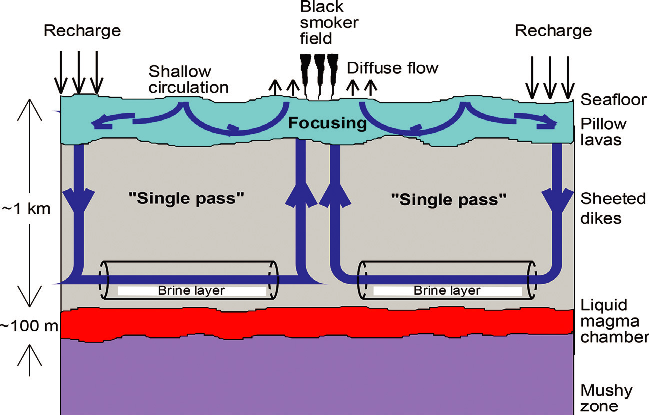
\includegraphics[width=\textwidth ]{SinglePassModel} 
	\caption[Single-pass model]{单通道模型} 
	\fnote{这是一段图注,乱按键盘:惊呆了撒娇来得及电路设计啊附近的骄傲而为的离开静安寺覅额黄飞鸿我积分对时间啊浪费我hi符合换个哈结尾覅哦啊见附件饿哦} 
	\label{fig:singlepassmodel} 
\end{figure} 

在这里引用此图,如图 \ref{fig:singlepassmodel} 所示。在论文末尾会自动生成插图索引。


\begin{figure} [htbp] 
	\centering
	
\includegraphics[width=0.5\textwidth ]{weixingongzhong} 
	\caption[Single-pass model]{Latex模板获取方法} 
	\fnote{扫码关注微信公众号并发消息\textcolor{red}{latex模板}即可获取模板文件} 
	\label{fig:template} 
\end{figure} 

在这里引用此图,如图 \ref{fig:singlepassmodel} 所示。在论文末尾会自动生成插图索引。

\subsection{表格}
表格与图类似,参见清华大学学位论文模板说明。

\subsection{公式}

行内公式,这个是行内公式 $E=MC^2$,下面是个带编号的独立公式:

\begin{equation}
	\frac{\partial T}{t} = \lambda \nabla T
	\label{eq:temperature}
\end{equation}

这里引用公式,公式\ref{eq:temperature}表示了温度的衰减。

\subsection{参考文献}
第一种引用方式:\cite{vehling2018implementation} 进行了相分离的数值模拟研究。
第二种引用方式:三维数值模拟目前仅限于单相流体\citep{coumou2008structure,coumou2006dynamics}。
这样的引用方式可能更易读一些,有可能地大要求以编号的形式显示,name只需要在main.tex里面把参考引用格式从{thuthesis-author-year}改为{thuthesis-numeric即可}
%%% 其它部分
\backmatter

%% 本科生要这几个索引,研究生不要。选择性留下。
% 插图索引
\listoffigures
% 表格索引
\listoftables
% 公式索引
%\listofequations


%% 参考文献
% 注意:至少需要引用一篇参考文献,否则下面两行可能引起编译错误。
% 如果不需要参考文献,请将下面两行删除或注释掉。
% 数字式引用
%\bibliographystyle{thuthesis-numeric}
% 作者-年份式引用
 \bibliographystyle{thuthesis-author-year}
\bibliography{ref/refs}


%% 致谢
%% 如果使用声明扫描页,将可选参数指定为扫描后的 PDF 文件名,例如:
% \begin{acknowledgement}[scan-statement.pdf]
\begin{acknowledgement}
  衷心感谢导师 xxx 教授和物理系 xxx 副教授对本人的精心指导。他们的言传身教将使
  我终生受益。

  在美国麻省理工学院化学系进行九个月的合作研究期间,承蒙 xxx 教授热心指导与帮助,不
  胜感激。感谢 xx 实验室主任 xx 教授,以及实验室全体老师和同学们的热情帮助和支
  持!本课题承蒙国家自然科学基金资助,特此致谢。

  感谢 \LaTeX 和 \thuthesis\cite{thuthesis},帮我节省了不少时间。
\end{acknowledgement}


%% 附录

\begin{appendix}
	\chapter{表格}


\begin{table}
	\centering
	\caption{数学符号和常数定义}
	\label{tab:append_Symbols_Values}
	\begin{tabular}{lcc}
		\toprule
		符号 & 定义 & 值/单位\tabularnewline
		\midrule
		$K$ & 渗透率 & $m^2$\\
		\bottomrule
	\end{tabular}
\end{table}


\end{appendix}

%% 个人简历
%\begin{resume}

  \resumeitem{个人简历}

  xxxx 年 xx 月 xx 日出生于 xx 省 xx 县。

  xxxx 年 9 月考入 xx 大学 xx 系 xx 专业,xxxx 年 7 月本科毕业并获得 xx 学士学位。

  xxxx 年 9 月免试进入 xx 大学 xx 系攻读 xx 学位至今。

  \researchitem{发表的学术论文} % 发表的和录用的合在一起

  % 1. 已经刊载的学术论文(本人是第一作者,或者导师为第一作者本人是第二作者)
  \begin{publications}
    \item Yang Y, Ren T L, Zhang L T, et al. Miniature microphone with silicon-
      based ferroelectric thin films. Integrated Ferroelectrics, 2003,
      52:229-235. (SCI 收录, 检索号:758FZ.)
    \item 杨轶, 张宁欣, 任天令, 等. 硅基铁电微声学器件中薄膜残余应力的研究. 中国机
      械工程, 2005, 16(14):1289-1291. (EI 收录, 检索号:0534931 2907.)
    \item 杨轶, 张宁欣, 任天令, 等. 集成铁电器件中的关键工艺研究. 仪器仪表学报,
      2003, 24(S4):192-193. (EI 源刊.)
  \end{publications}

  % 2. 尚未刊载,但已经接到正式录用函的学术论文(本人为第一作者,或者
  %    导师为第一作者本人是第二作者)。
  \begin{publications}[before=\publicationskip,after=\publicationskip]
    \item Yang Y, Ren T L, Zhu Y P, et al. PMUTs for handwriting recognition. In
      press. (已被 Integrated Ferroelectrics 录用. SCI 源刊.)
  \end{publications}

  % 3. 其他学术论文。可列出除上述两种情况以外的其他学术论文,但必须是
  %    已经刊载或者收到正式录用函的论文。
  \begin{publications}
    \item Wu X M, Yang Y, Cai J, et al. Measurements of ferroelectric MEMS
      microphones. Integrated Ferroelectrics, 2005, 69:417-429. (SCI 收录, 检索号
      :896KM)
    \item 贾泽, 杨轶, 陈兢, 等. 用于压电和电容微麦克风的体硅腐蚀相关研究. 压电与声
      光, 2006, 28(1):117-119. (EI 收录, 检索号:06129773469)
    \item 伍晓明, 杨轶, 张宁欣, 等. 基于MEMS技术的集成铁电硅微麦克风. 中国集成电路,
      2003, 53:59-61.
  \end{publications}

  \researchitem{研究成果} % 有就写,没有就删除
  \begin{achievements}
    \item 任天令, 杨轶, 朱一平, 等. 硅基铁电微声学传感器畴极化区域控制和电极连接的
      方法: 中国, CN1602118A. (中国专利公开号)
    \item Ren T L, Yang Y, Zhu Y P, et al. Piezoelectric micro acoustic sensor
      based on ferroelectric materials: USA, No.11/215, 102. (美国发明专利申请号)
  \end{achievements}

\end{resume}


%% 本科生进行格式审查是需要下面这个表格,答辩可能不需要。选择性留下。
% 综合论文训练记录表
%\includepdf[pages=-]{scan-record.pdf}
\end{document}
